\begin{figure}[H]
        \centering 
        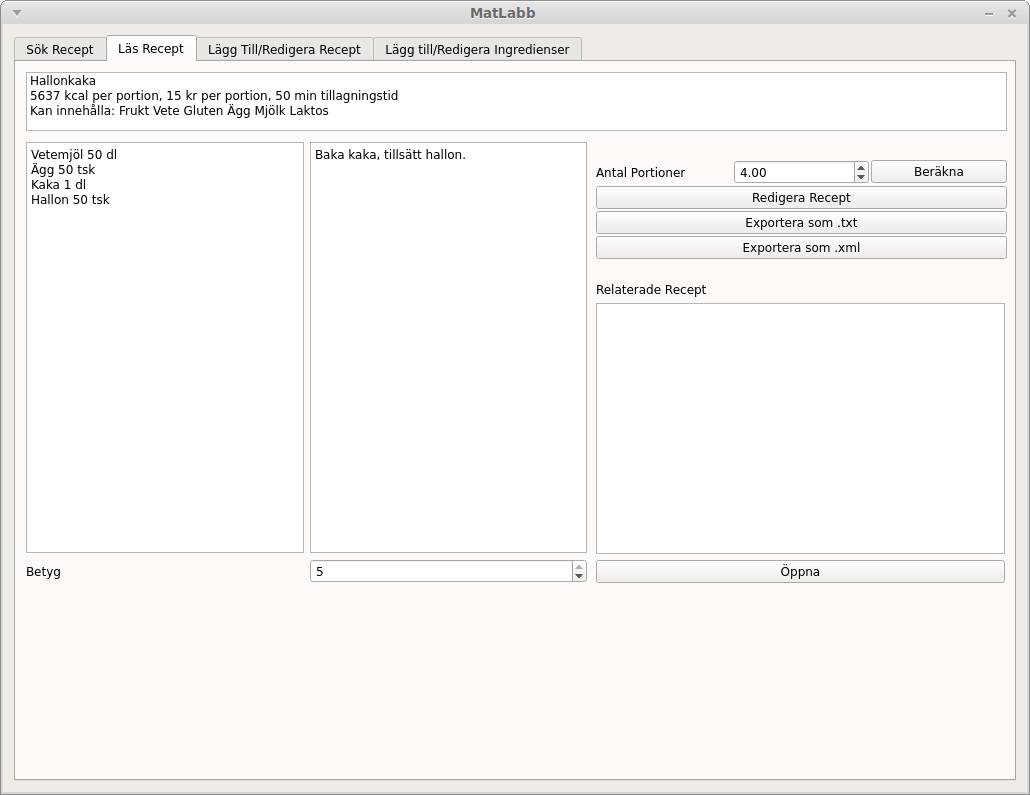
\includegraphics[scale=0.44]{las_recept.png} 
        \caption{Läs receptvyn} 
        \label{fig:receptvyn}
\end{figure}

I \verb+Läs recept+-vyn möts man av en rad fält. I huvudfältet längst upp finner
man information om receptets namn antal kilokalorier per portion,
antal kronor per portion och hur lång tid receptet tar att laga.

Under huvudfönstret finns från vänster sett Ingrediensfältet,
instruktionsfältet samt portionsskalning och knappar för imort/exort
och redigering . I ingrediensfältet finns de ingredienser som krävs
samt åtgångsmängd, i instruktionsfältet hittar man de instruktioner
som behövs för att tillaga maträtten.

Till höger om instruktionsfältet finns portionsskalaren. Med pilarna
kan antalet portioner ändras och när knappen \verb+beräkna+ trycks in
skalas receptet om. Under knapparna för redigering och export finns en
lista över relaterade recept som kan öppnas med knappen \verb+öppna+.

Nederst i fönstret kan receptets betyg öppnas med pilarna.
